%To generate pdf:
%pdflatex description.tex

\documentclass{article}

\usepackage[letterpaper, margin=0.5in]{geometry}
\usepackage{graphicx} % Required to insert images
\usepackage{epstopdf}
\usepackage{listings} % Required for insertion of code
\usepackage{amssymb,amsmath}

\setlength{\parindent}{0pt}
\setlength{\parskip}{1ex}

\begin{document}

\title{Problem Description for Diffusion Through Nanopore}
\author{Tom Pace}
\maketitle

%-------------------------------------------------------------------------------
\section{Background}

We study a silica membrane containing nanoscopic circular pores arranged in a two-dimensional lattice.
We desire to understand the rate of transport of different ions through the nanopores,
quantified in terms of an effective diffusion constant.
The pore geometry is variable, as is the diffusion equation governing transport.

%-------------------------------------------------------------------------------
\section{System Geometry}

We study both a body-centered rectangular lattice of pores,
as well as a face-centered lattice of pores.
The unit cell geometry has two planes of symmetry.
This symmetry is used to reduce the model to only one quarter of the unit cell.

The geometry and geometric variables are shown below.

\textbf{TODO: get figure numbers for reference in text}

\begin{figure}[htbp]
\centering
\includegraphics[height=0.50000\textwidth]{./fig_pdf/body-top.pdf}
\caption{Top view of body-centered geometry}
\end{figure}

\begin{figure}[htbp]
\centering
\includegraphics[height=0.50000\textwidth]{./fig_pdf/body-side.pdf}
\caption{Side view of body-centered geometry}
\end{figure}

$\begin{array}{rcl}
Sx & = & 2 Lx =\text{Unit cell x-dimension} \\
Sy & = & 2 Ly =\text{Unit cell y-dimension} \\
Lx & = & \frac{Sx}{2} =\text{Model x-dimension} \\
Ly & = & \frac{Sy}{2} =\text{Model y-dimension} \\
R & = & \text{Pore radius} \\
tm & = & \text{Membrane thickness} = \text{Pore length} \\
H & = & \text{Distance from membrane surface to model boundary}
\end{array}$



\textbf{TODO: body-centered side view is incomplete}

\textbf{TODO: consider combining views into one image horizontally}

\textbf{TODO: face-centered geometry, both views}

%-------------------------------------------------------------------------------
\section{Diffusion Equation}

\subsection{Unhomogenized Standard Diffusion Equation}

\subsection{Homogenized Standard Diffusion Equation}



\textbf{TODO}

\end{document}
